\documentclass{jarticle}

\usepackage{tam}
\usepackage{fleqn}
\usepackage{url}
\usepackage{bm}
\usepackage[dvipdfmx]{graphicx}
\usepackage[dvipdfmx]{color}
%\usepackage{color}
\usepackage{colordef}
\usepackage{amssymb}
\usepackage{pdfpages}
\usepackage{amsmath}

%%%%%%%%%% Command alias %%%%%%%%%%
\newcommand{\IB}{$\bullet$}
\newcommand{\IC}{$\circ$}
\newcommand{\IS}{$*$}
%%%%%%%%%%%%%%%%%%%%%%%%%%%%%%%%%%%

\title{動的計画法を用いた電力運用最適化}
\author{神戸大学大学院 奥村侑真}
\date{}

\def\baselinestretch{1.02}
\renewcommand{\thefootnote}{\roman{footnote}}

\begin{document}
\maketitle

\section{はじめに}
図\ref{fig:tecseed}に示す電力ネットワークに対する，電力クラスタの電力運
用最適化モデルを示す．

\begin{figure}[h]
 \centering
 
\includegraphics[width=155mm]{../tecseed.pdf}
 \caption{テクシード構成図}
 \label{fig:tecseed}
\end{figure}

\section{準備}

基本要素およびそのスペックを表す定数(\IB を付して記す)と状態変数(\IC を付
して表す)として以下のものを用意する．

%\begin{itemize}
% \item[$\triangleright$] 電力クラスタC$_{i}$ $(i=1,\ldots,N)$:
\begin{itemize}
 \item[\IS] 期T$_k$ ($k=1,\ldots,K$)．本検証では各期の幅は$60$秒としている．
 \item[\IS] 太陽光発電機G
 \item[\IS] 消費機器D$^{\rm A}$
 \item[\IS] 消費機器D$^{\rm B}$
 \item[\IS] 消費機器D$^{\rm C}$
 \item[\IS] 固定バッテリーB$^{\rm F}$
  \begin{itemize}
   \item[\IB] 固定バッテリーの容量 $\overline{b}$
  \end{itemize}
 \item[\IS] 電力変換器(太陽光) E$^{\rm P}$
  \begin{itemize}
   \item[\IB] 変換効率 $\alpha^{\rm P}$

  \end{itemize}
 \item[\IS] 電力変換器(系統電力) E$^{\rm S}$
 \item[\IS] 電力変換器(消費機器A) E$^{\rm A}$
  \begin{itemize}
   \item[\IB] 変換効率 $\alpha^{\rm DA}$
  \end{itemize}
 \item[\IS] 電力変換器(消費機器B) E$^{\rm B}$
  \begin{itemize}
   \item[\IB] 変換効率 $\alpha^{\rm DB}$
  \end{itemize}
 \item[\IS] 電力変換器(消費機器C) E$^{\rm C}$
  \begin{itemize}
   \item[\IB] 変換効率 $\alpha^{\rm DC}$
  \end{itemize}
 \item[\IS] 電力変換器(固定バッテリー)E$^{\rm BF}$
  \begin{itemize}
   \item[\IB] 充電効率 $\alpha^{\rm FC}$
   \item[\IB] 放電効率 $\alpha^{\rm FD}$
   \item[\IB] 自己放電効率 $\alpha^{\rm FT}$
  %\item[\IB] 単位時間あたりの最大充電電量 $a^{\rm FC}$
  %\item[\IB] 単位時間あたりの最大充放電量 $a^{\rm FD}$
  \end{itemize}
 \item[\IS] 系統電力S
   \begin{itemize}
   \item[\IB] 系統買電単価 $p^{\rm BY}_{k}$
   \item[\IB] 単位時間あたりの最大系統買電量 $a^{\rm BY}$
   \item[\IB] 系統売電単価 $p^{\rm SL}_{k}$
   %\item[\IB] 単位時間あたりの最大系統売電量 $a^{\rm SL}_{k}$
  \end{itemize}
\end{itemize}

\section{定数・変数 \mbox{\normalsize\rm 
~ (定数を「\IB」，変数を「\IC」を付して記すものとする)}}

 \begin{itemize}
  \item[\IB] 太陽光発電電力量(変換前) $g^{\rm P1}_{k}$
  %\item[\IC] 太陽光発電電力量(変換後) $g^{\rm P2}_{k}$
  %\item[\IC] ムダ電力量 (太陽光発電出力抑制量)$v_{k}$ \\[-2.5ex]
  %
  %\item[\IC] 消費電力A (変換前) $d^{\rm A1}_{k}$
 \item[\IB] 消費電力A (変換後) $d^{\rm A2}_{k}$
  %
  %\item[\IC] 消費電力B (変換前) $d^{\rm B1}_{k}$
  \item[\IB] 消費電力B (変換後) $d^{\rm B2}_{k}$
  %
 % \item[\IC] 消費電力C (変換前) $d^{\rm C1}_{k}$
  \item[\IB] 消費電力C (変換後) $d^{\rm C2}_{k}$
  %
  \item[\IB] 固定バッテリーのSOCの初期段階 $i_{0}$
  \item[\IB] 固定バッテリーのSOCを離散化したときの分割数$B$
  \item[\IC] 固定バッテリーの(期末の)SOC $b^{\rm F}_{k}$
  %\item[\IC] 固定バッテリーの充電量(変換前) $x^{\rm FC1}_{k}$
  %\\ただし，$x^{\rm FC1}_{k}がx^{\rm FC1}_{k} < 0$を満たしているときは$|x^{\rm FC1}_{k}|$だけ放電を行っていると解釈する．
  \item[\IC] 固定バッテリーの充電量(変換後) $x^{\rm FC2}_{k}$
   \\ただし，$x^{\rm FC1}_{k}がx^{\rm FC2}_{k} < 0$を満たしているときは$|x^{\rm FC2}_{k}|$だけ放電を行っていると解釈する．
  %\item[\IC] 固定バッテリーの放電量(変換前) $x^{\rm FD1}_{k}$
  %\item[\IC] 固定バッテリーの放電量(変換後) $x^{\rm FD2}_{k}$ \\[-2.5ex]

  %
  \item[\IC] 系統買電力量$s^{\rm BY}_{k}$  \\ただし，$s^{\rm BY}_{k}がs^{\rm BY}_{k} < 0$を満たしているときは$|s^{\rm BY}_{k} |$だけ系統に売電を行っていると解釈する．
  %\item[\IC] 系統売電力量$s^{\rm SL}_{k}$
  
  %\item[\IC] 系統電力量(変換前)$s^{1}_{k}$．
  %\item[\IC] 系統電力量(変換後)$s^{2}_{k}$．
  %\item[\IB] 変換効率$\alpha^{\rm S}$．
  %
\end{itemize}


\section{動的計画法によるアプローチ}
\subsection{定式化}
前節で示した定数・変数を用いて，電力運用最適化問題に対して動的計画法を用いたアプローチを検討する．
まず，バッテリーのSOCとしてとりうる値を，0が最小値となり $\overline{b}$が最大値となるように，等間隔に $B( \geq 2)$段階で離散化する．これにより，期 \(k\) の末尾におけるSOCは以下の \(B\) 個の値のいずれかをとる：
\[
0,\ \frac{1}{B-1}\overline{b},\ \frac{2}{B-1}\overline{b},\ \dots,\ \overline{b}．
\]
便宜上，期 $k$ の末尾においてSOCが $\frac{i}{B-1}\overline{b}$である状態を，「バッテリーのSOCが $i$ 段階である」と呼ぶことにする$(i=0,1,\dots ,  B - 1)$．

次に，期ごとの状態を要素に持つ集合$S_{0},S_{1},\dots,S_{K-1}$を以下のように定義する：
\begin{equation}
S_k = \begin{cases}
  \left\{  s_{i_0}  \right\} ,\quad \text{if } k = 0 \\
  \left\{ s_{i} \mid i = 0, 1, \dots, B - 1 \right\} ,\quad \text{if } 1 \leq k \leq K．
\end{cases}
 \label{eq:state}
\end{equation}

ここで，状態$s_{i}( \in S_{k})$ は，期 $k$におけるSOCが$i$段階である状態を表す．

%各状態 $ s_{i} (\in S_{k})$に対応する評価値を $F_{k}(s_{i})$，
状態 $s_{i}(\in S_{k-1})$から$ s_{j} (\in S_{k})$への遷移に伴う評価関数を$w_{k-1}(s_{i},s_{j})$とする．このとき，問題は以下のように定式化される．
\begin{equation}
    \text{Minimize} \quad \{ \sum_{i=0}^{K-1} w_i(s_j,s_k) | s_j \in S_i, s_k \in S_{i+1} \}
 \label{eq:minimize}
\end{equation}


以下評価関数の計算方法について述べる．評価関数 $w_{k-1}(s_{i},s_{j})$は以下で与えられる：
\begin{equation}
  %w_{k-1}(s_{i},s_{j}) = p_k^{\rm BY/SL} \left[ \frac{j - i}{n-1} \cdot \overline{b} - \{ g_k^{\rm P2} - (d_k^{\rm A2} + d_k^{\rm B2} + d_k^{\rm C2}) \} \right]．
  w_{k-1}(s_{i},s_{j}) = \begin{cases}
   p_k^{\rm BY}s_k^{\rm BY} ，  \text{if }  s_k^{\rm BY}  \geq 0\\
   p_k^{\rm SL}s_k^{\rm BY} ，\text{otherwise}．
   \end{cases}
 \label{eq:weight}
\end{equation}


ここで，
\begin{equation}
 s_k^{\rm BY} = \begin{cases}
 \frac{d_k^{\rm A2}}{\alpha^{\rm DA}} + \frac{ d_k^{\rm B2}}{\alpha^{\rm DB}} + \frac{ d_k^{\rm C2}}{\alpha^{\rm DC}}+  \frac{x_k^{\rm FC2}}{\alpha^{\rm FC}} - \alpha^{\rm P}  g_k^{\rm P1} ，\text{if}(x_k^{\rm FC2} \geq 0) \\
 
  \frac{d_k^{\rm A2}}{\alpha^{\rm DA}} + \frac{ d_k^{\rm B2}}{\alpha^{\rm DB}} + \frac{ d_k^{\rm C2}}{\alpha^{\rm DC}}+  \alpha^{\rm FD}x_k^{\rm FC2} - \alpha^{\rm P}  g_k^{\rm P1} ，\text{otherwise}
 
 \end{cases}
 \label{eq:pass}
\end{equation}
が成立する．また，ある期の末からその1期次の期の末までのバッテリーの変化量に注目すると，

\begin{equation}
 x_k^{\rm FC2} =  \frac{j - i}{B-1} \overline{b}
 \label{eq:BF}
\end{equation}
となるので，(\ref{eq:pass})，(\ref{eq:BF})より，

\begin{equation}
 s_k^{\rm BY} = \begin{cases}
 \frac{d_k^{\rm A2}}{\alpha^{\rm DA}} + \frac{ d_k^{\rm B2}}{\alpha^{\rm DB}} + \frac{ d_k^{\rm C2}}{\alpha^{\rm DC}}+  \frac{1}{\alpha^{\rm FC}}\frac{j - i}{B-1} \overline{b} - \alpha^{\rm P}  g_k^{\rm P1} ，\text{if}(\frac{j - i}{B-1} \overline{b} \geq 0) \\
 
  \frac{d_k^{\rm A2}}{\alpha^{\rm DA}} + \frac{ d_k^{\rm B2}}{\alpha^{\rm DB}} + \frac{ d_k^{\rm C2}}{\alpha^{\rm DC}}+  \alpha^{\rm FD}\frac{j - i}{B-1} \overline{b} - \alpha^{\rm P}  g_k^{\rm P1} ，\text{otherwise}
 
 \end{cases}
 \label{eq:SBY}
\end{equation}
がいえる．(\ref{eq:SBY})の右辺に現れる全ての文字は既知であるため，(\ref{eq:weight})の右辺に現れる全ての文字は既知となる．よって，任意の$i,j,k(0\leq k \leq K)$について，状態 $s_{i}(\in S_{k-1})$から$ s_{j} (\in S_{k})$への遷移に伴う評価関数$w_{k-1}(s_{i},s_{j})$を設定することができる．

モデル中の定数・変数と電力クラスタとの関係を図\ref{fig:tecseed}に示す．

\begin{figure}[h]
 \centering
 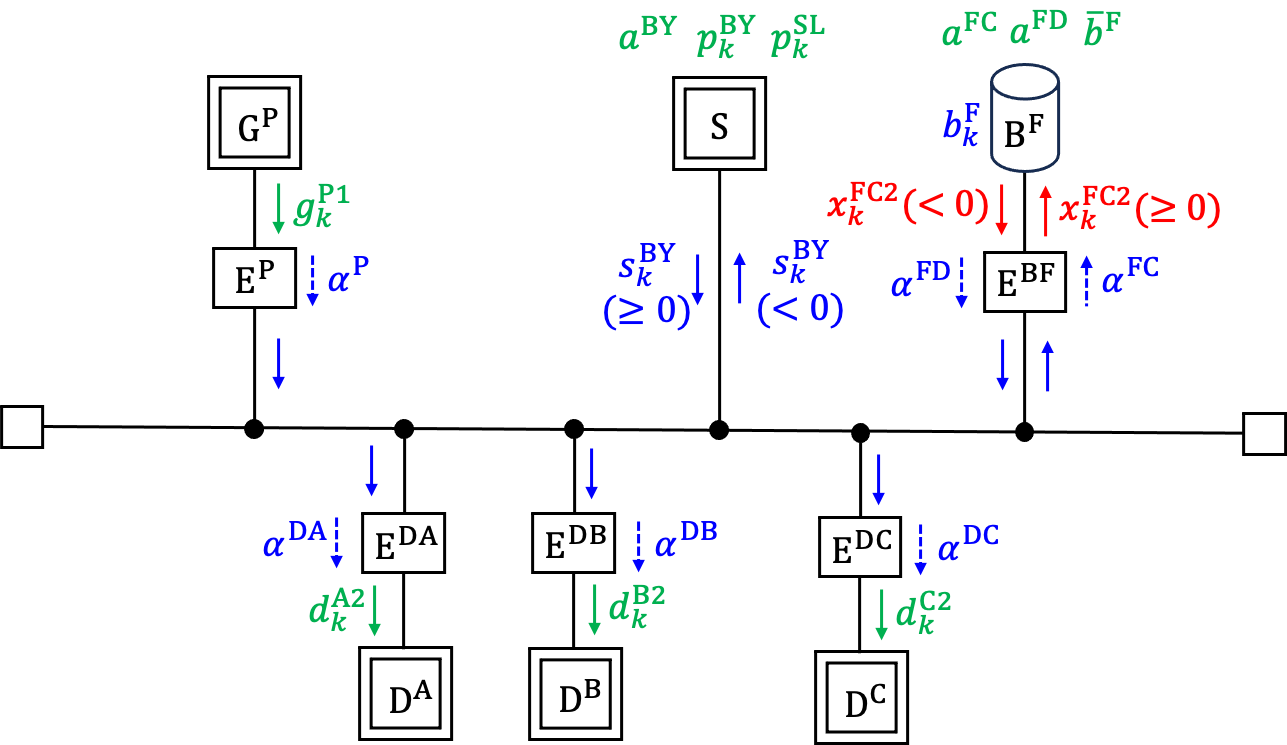
\includegraphics[width=140mm]{../figure/tecseed20250904.png}
 \caption{電力クラスタの構成図 (\textcolor{red}{赤: 決定変数}，\textcolor{blue}{青: 従属変数}，\textcolor{green3}{定数(外生変数)})}
 \label{fig:tecseed}
\end{figure}

\subsection{最適性の原理と更新式}
本問題は，「最適経路の部分経路もまた最適でなければならない」という最適性の原理を満たしており，動的計画法により解くことができる．最適性の原理を満たすことの証明は4.4.で述べる．
動的計画法による更新式は以下の通りで表される：
\[
F_{0}(s_{i_{0}}) = 0 ,\quad \text{if } k = 0 \\
\]
\[
F_{k}(s_{i}) = \min_{s_{j} \in S_{k-1}} ( F_{k-1}(s_{j}) + w_{k-1}(s_{j},s_{i}) )  ,\quad (1 \leq k \leq K) \\
 ．
 \label{eq:minimize}
\]
この更新式に則って $F_{0}$ から $F{K}$ まで順次に値を求めることで，最終的な状態における最小の評価値と，その最小の評価値を得るためには，各々の期でどのように状態を遷移すればよいのかを求めることができる．


\subsection{バッテリーの刻み幅} 
 本アプローチにおける計算量は，$O(B^2 K)$となる．
$K$についてはフードテクノ株式会社様から「2週間程度の電力運用計画をつくりたい」という要望があり調節をすることができないため，
現実的な計算時間内で最適な解を得るためには，バッテリーの段階の個数である$B$をどの程度の大きさに設定するかが肝要となる． 
 フードテクノ株式会社から「30分間のデマンド電力が50kW以下という制約条件を加えたい」という要求があるため，$B$の値が小さすぎる場合，
 30分間のデマンド電力が50kW以下になるような状態遷移が存在しなくなってしまうことがある．逆に，$B$の値が大きすぎる場合，計算時間が大きくなりすぎてしまう．
これらを考慮した$B$の設定例の1つとして，バッテリーの1段階あたりの刻み幅が$0.4$ kWh となるように$B$を設定することを考えた．この値であれば，全ての期について，系統からの買電を行う状態遷移が少なくとも1つ存在することが保証される．
また，バッテリー容量は$\overline{b}=2742$ kWhであるため，このとき$B$の値は6855となる．

\subsection{最適性の原理の証明}
背理法によって証明できる．期 $k-1$ の状態 $s_j$ を経由して期 $k$ の状態 $s_i$ に至るある最適経路($F_k(s_i)$が最小になるような経路) $P^*$ があったとする．このとき，その部分経路である期 $k-1$ の状態 $s_j$ に至るまでの経路 $P^*_{0 \to k-1}$ が最適でなかったと仮定する．
このとき，状態 $s_j$ に至るまでにより最適な別の経路 $P'$ が存在し，その評価値を $F'_{k-1}(s_j)$ とすると，$F'_{k-1}(s_j) < F_{k-1}(s_j)$ が成り立つ．
また，経路 $P'$ を通り，そこから状態 $s_i$ へ遷移する新しい経路を構成すると，その評価値は $F'_{k-1}(s_j) + w_{k-1}(s_j, s_i)$ となる．これは，仮定した最適経路 $P^*$ の評価値$F_{k-1}(s_j) + w_{k-1}(s_j, s_i)$ よりも小さくなる．
これは，経路 $P^*$ が最適であるという当初の仮定と矛盾する．
したがって，最適経路の部分経路もまた最適でなければならない．

\end{document}
